\chapter{Liquid-State Overhauser DNP}
\label{chap:overhauser}

Continuous-wave (CW) Overhauser dynamic nuclear polarization transfers
electron polarization to solvent nuclei through stochastic electron--nuclear
interactions. Use \code{spin\_dynamics.dnp} for homogeneous liquid-state
spin-1/2 targets with positive gyromagnetic ratio. This model is distinct from
parahydrogen spin order and from a prescribed polarization multiplier.

\chapterpath{Choose molecular-motion rates or measured factors, calculate
nitroxide saturation, distinguish solution ensembles from a closed spin pair,
and reproduce the published TEMPOL comparisons.}

\section{Rates, Signs, and the Shortest Calculation}

The baseline-inclusive enhancement and its factors are
\[
 E=\frac{P_n}{P_n^0}=1-\xi f s\frac{|\gamma_e|}{\gamma_n},\qquad
 \xi=\frac{R_\sigma}{R_\rho},\quad
 f=\frac{R_\rho}{R_{10}+R_\rho}.
\]
Positive cross relaxation inverts the proton enhancement. Gyromagnetic ratios
are positive magnitudes in Hz/T, spectral frequencies are angular frequencies,
rates are in s$^{-1}$, and concentration is mol/L. Published enhancement
\(\epsilon=(M_{\rm on}-M_{\rm off})/M_{\rm off}\) equals \(E-1\).

\begin{lstlisting}[language=Python]
from spin_dynamics.dnp import (
    TranslationalDiffusionModel, translational_relaxation_rates,
    cw_overhauser, polarization_buildup,
)
motion = TranslationalDiffusionModel(0.39e-9, 2.8e-9)
rates = translational_relaxation_rates(
    0.35, motion, concentration_molar=0.005,
    background_r1_per_second=1/2.5,
)
cw = cw_overhauser(rates, field_tesla=0.35, saturation_factor=0.8)
trajectory = polarization_buildup(cw, [0, 0.1, 1, 5])
print(cw.enhancement, cw.steady_state_polarization, cw.rates.t1_seconds)
\end{lstlisting}

These diffusion and saturation parameters are illustrative. Force-free
hard-sphere translation uses \(\tau_D=d^2/D_{\rm relative}\) and a normalized
one-sided spectral density. Zero frequency gives \(J(0)=4\tau_D/9\).

\code{MotionBasedCWModel} adds independent translational, rotational-dipolar
and fluctuating scalar-contact channels. Bound-pair counts are not radical
molarity. The same population must not be counted in two motion channels.
Measured T1, relaxivities, or coupling/leakage/saturation factors are supported
separately. Temperature-dependent transport and microwave heating must be
supplied; they are not inferred from the radical name.

\section{Nitrogen Hyperfine Saturation}

Saturating one resolved nitroxide line does not generally saturate the electron
ensemble. Without interline transfer, selective irradiation approaches effective
saturation of 1/3 for nitrogen-14 or 1/2 for nitrogen-15. Nitrogen relaxation and
Heisenberg exchange transfer saturation between lines.

\begin{lstlisting}[language=Python]
from spin_dynamics.dnp import NitroxideSaturationModel
model = NitroxideSaturationModel(
    electron_t1_seconds=[0.4e-6, 0.5e-6, 0.6e-6],
    electron_t2_seconds=[80e-9, 100e-9, 130e-9],
    nitrogen_transition_per_second=1e4,
    exchange_coefficient_per_molar_second=2e9,
    transverse_broadening_per_molar_second=1e9,
)
sat = model.steady_state(field_tesla=0.35,
    concentration_molar=0.005, nutation_rad_per_s=20e6)
print(sat.saturation_factor, sat.nitrogen_populations)
\end{lstlisting}

Line vectors are ordered by ascending nitrogen projection. Exchange frequency
is \(k_{ex}=K_{ex}C\), defined as population-correlation decay; transverse
broadening adds a separately supplied coefficient times concentration to R2.
Other literature rate conventions can differ by numerical factors.

For the full treatment, \code{NitroxideRelaxationMatrix} contains a
\((2n,2n)\) population loss block and an \((n,n)\) transverse relaxation block.
Its isotropic-tumbling factory uses aligned g and hyperfine principal tensors,
their covariance, spin-rotation spectra, and additional electron relaxation.
The generalized Bloch solver retains R1, R2, R0, U and V, including nitrogen
population feedback and transverse exchange transfer. Supply
\code{relaxation\_matrix=...} and set the independent T1/T2 to positive infinity
when those baths are already in the supplied operator. Independent and matrix
contributions are additive. A symmetric nitrogen loss matrix can also specify
arbitrary spin-independent transfer networks. Loss matrices have nonpositive
off-diagonal entries and zero sums.

Full mode solves first-order high-temperature deviations about a factorized
thermal reference, with linearized exchange. It is not finite-temperature
Gibbs propagation. Nuclear quadrupolar coherences, nonsecular shifts and
general coalescence remain outside this model. The default scalar population
path retains its original nonlinear-swap approximation. Effective saturation
uses total electron polarization, including nonuniform nitrogen populations.

\section{Pair Dynamics and Solution Ensembles}

\code{CoupledElectronNuclearModel} instead treats one electron and one target
nucleus. It provides laboratory-gap detailed-balance jumps, finite-temperature
Gibbs recovery, coherent microwave driving, stationary states and trace-preserving
propagation. Its 1:1 population mapping is not the electron-to-proton number
density of a dilute radical solution. Bulk nuclear relaxivities alone cannot
specify the corresponding electron bath. Do not insert solution-averaged FFHS
rates into a closed pair and interpret it as an entire sample.

\section{Reproduction and Evidence}

Run from \code{PythonSpinDynamics}:
\begin{lstlisting}[language=bash]
python examples/plot_overhauser_tempol_saturation.py --output .tmp/tempol.png
python examples/plot_overhauser_coupled_dynamics.py --output .tmp/pair.png
python examples/plot_tempol_published_benchmarks.py --output .tmp/published.png
python validation/validate_tempol_water.py
python validation/validate_overhauser_diffusion.py
\end{lstlisting}

The published benchmark compares unchanged extracted TEMPOL/water observations
with three model stages. No enhancement fitting is performed.
\begin{center}
\begin{tabular}{@{}lrr@{}}
\toprule
Model & DNP RMSE & Saturation-theory RMSE \\
\midrule
Common-T2 population reduction & 0.48285 & 0.01751 \\
Line-dependent T2 population model & 0.47456 & 0.01923 \\
Full nitrogen relaxation and exchange & 0.48849 & 0.01657 \\
\bottomrule
\end{tabular}
\end{center}
The full operator improves the theory comparison but slightly worsens the
measured DNP comparison. Agreement is partial; digitization precision is not
measurement uncertainty. The saturation profile is published theory, and
lower-field saturation anchors were inferred from DNP rather than measured
independently. A separate reconstructed EPR-fit comparison exposes a 4.32-fold
cross-study difference in relaxation-time products. It is not a universal
TEMPOL calibration. Source locations, native pixels and checksums are retained
in \code{validation/experimental/tempol\_water\_published.json}.

\begin{figure}[p]
\centering
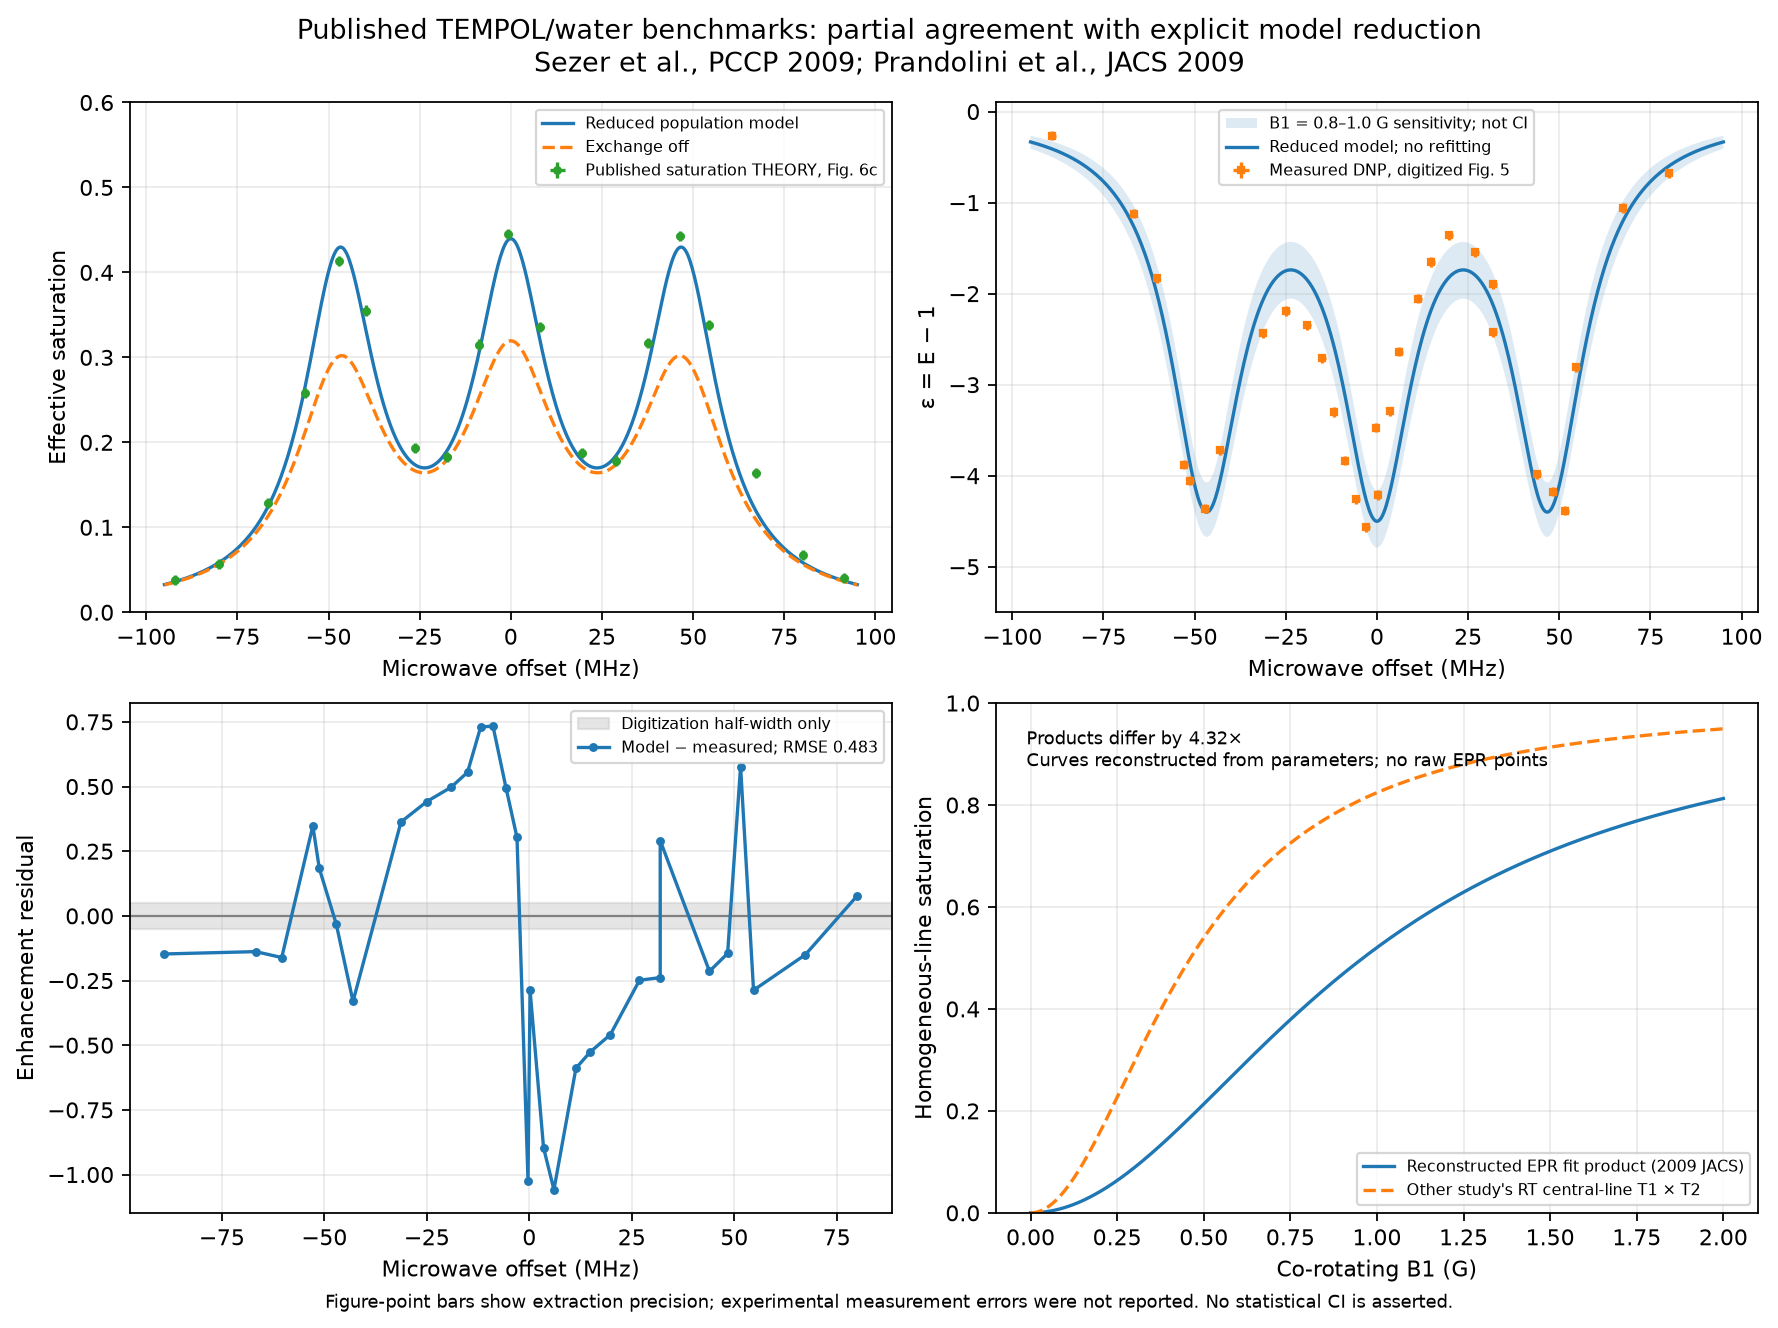
\includegraphics[width=0.98\linewidth]{assets/tempol_published_comparison.png}
\caption{Published TEMPOL/water comparisons. Full and reduced relaxation
models are shown against experimental DNP markers, published saturation
theory and a reconstructed EPR saturation fit. These are different evidence
types; the shaded B1 range is sensitivity, not a confidence interval.}
\label{fig:tempol-published}
\end{figure}

The searchable \href{https://supertjhok.github.io/MRSpinDynamics/overhauser_dnp/}{CW
Overhauser guide} contains full API examples and conventions. The companion
\href{https://supertjhok.github.io/MRSpinDynamics/tempol_published_benchmarks/}{benchmark
guide} records extraction and model limitations.
